\documentclass[11pt]{amsart}
\usepackage{geometry}                % See geometry.pdf to learn the layout options. There are lots.
\geometry{letterpaper}                   % ... or a4paper or a5paper or ... 
%\geometry{landscape}                % Activate for for rotated page geometry
%\usepackage[parfill]{parskip}    % Activate to begin paragraphs with an empty line rather than an indent
\usepackage{graphicx}
\usepackage{amssymb}
\usepackage{epstopdf}
\usepackage{subfig}
\DeclareGraphicsRule{.tif}{png}{.png}{`convert #1 `dirname #1`/`basename #1 .tif`.png}
\bibliographystyle{abbrv}

\title{Identifying Structure in Gradable Adjectives Through Corpus Analysis}
\author{Kevin Leung}
\thanks{This project was done with Daniel Lassiter, a postdoc in the CoCo Lab. Dan motivated the project and provided qualitative, linguistic analysis. I was responsible for the technical approach, implementation, and quantitative analysis.}

%\date{}                                           % Activate to display a given date or no date

\begin{document}
\maketitle

Many of human concepts can be expressed in varying degrees, and in English, we can express these using gradable adjectives. Gradable adjectives accept degree modifiers, which determine the strength of the concept being expressed. For example, "tall" is a gradable adjective because one can be "very tall" or "kind of tall." On the other hand, "dead" is a non-gradable adjective because one cannot be "very dead" or "slightly dead." Different gradable adjectives, however, accept different degree modifiers, and Kennedy and McNally\cite{kennedymcnally} offer a theory that types of gradable adjectives are determined by their scale structures.

In this project, we explore methods to evaluate this theory through corpus analysis. Specifically, we pick out instances of adverbial modification and analyze the frequency of different degree modifiers with adjectives. We compare clusterings over the distribution of degree modifier frequency with predicted groupings from the Kennedy and McNally theory to evaluate the theory. As an exploratory project, we consider multiple methods for each step and analyze the results to determine which methods works best.

\section{Kennedy and McNally Theory of Gradable Adjectives}
The theory offered by Kennedy and McNally\cite{kennedymcnally} is that gradable adjectives accept degree modification according to the scale structure that they fit. A scale is a total ordering over degrees for the concept being expressed by an adjective. These scales come in various types depending on whether they have minimum and maximum values. Thus, a scale can be open (no minimum or maximum), closed (minimum and maximum), lower closed (only minimum), and upper closed (only maximum). These correspond to different possible degree modifiers that they accept. For example, proportional modifiers work with adjectives with closed scales.

\begin{enumerate}
\item Alden thought the football stadium was half full.
\item ?? Maneesh bought a half expensive shirt.
\end{enumerate}

Another example of a scale-constrained modifier is \textit{slightly}, which relates to a minimum value.

\begin{enumerate}
\item Gabor rode his bike on the slightly wet road.
\item ?? Chris made many slightly accurate comments during class.
\end{enumerate}

Scale structures are important in human reasoning, and this theory has consequences on how language shapes thought.

\section{Related Work}
Rooth et al.\cite{rooth} implemented a EM-based clustering algorithm on co-occurrence frequencies in large corpora to discover semantic classes. Boleda Torrent and Alonso i Alemany\cite{boleda} used clustering to find adjective classes in Catalan based on several simple features, including the POS within a five-word window and a few handwritten rules. Hatzivassiloglou\cite{hat} tested several methods of extracting noun-adjective relationships from a corpus and clustered those result to find semantic classes for adjectives. Syrett and Lidz\cite{syrett} did a small corpus analysis to find a difference in degree modification of open and closed scale gradable adjectives to show that there are usage differences for children to observe and learn from.

\section{Overview of the Approach}
Our approach to evaluating the Kennedy and McNally theory was broken up into 3 general tasks, each of which will be explained and analyzed separately. 

First, we looked for appropriate corpora and extract frequencies to analyze. The two primary approaches used here were bigram counts and dependency counts of adverbial modification. Second, we considered different metrics for working with these counts, trying to extract more of the properties we felt were important from a potentially sparse, varied, and noisy dataset. Finally, we applied different clustering algorithms and evaluated the results against predicted clusters from the theory.

After discussing each of these steps below, we will provide a more general error analysis and discussion for future work.

\section{Data}
To narrow all of the possible adjectives and adverbs to consider, we took the 1000 most common words and picked out all of the adjectives and adverbs from that set. These were further trimmed down to a set of 135 adjectives (both gradable and non-gradable) and 41 adverbs (mostly degree modifiers) that were used in most of our analysis. Although all analysis should generalize to larger sets, we limited ourselves to this smaller set so that we could more easily analyze the data by hand.

We tried 2 different methods of counting instances of degree modification: bigrams and dependencies. Bigrams were simply the frequency of a word from our modifier set appearing before a word from our adjective set. We used the Stanford Parser\cite{marneffe} to find dependencies and couned up all instances of adverbial modification.

Most of the following analysis was done on the Web 1T corpus with over 1 trillion tokens extracted on the internet. This gave us just under 300 million bigram instances to consider. Unfortunately, Web 1T doesn't offer a dependency parse or any context for these instances.

The second corpus we used was English Gigaword, which was collected from 4 international newswire services. This contained about 1.75 billion tokens. Although we were able to extract some data from it, we unfortunately ran into memory problems parsing it (even with 4gb allocations). In all, we were only able to parse through approximately 100 million tokens. This resulted in only a total of approximately 6,000 instances of both bigrams and dependencies, which was far too sparse for our matrix with 5,535 cells. We compared the results of the bigram and dependencies on Gigaword to find how much these diverged but did not use the data in following steps.

\subsection{Results and Analysis}
Since we were only capable of using the results from Web 1T bigrams, our analysis in this step focused on whether there was an appreciable difference using these 2 methods. Turning the frequency matrix into a vector, there was a cosine similarity of .984 between the bigrams and dependencies. Strictly from a high-level quantitative perspective, it appears that these 2 methods were very similar.

Looking more closely at the examples, the results were mostly similar. A rough count over a small set showed that there was about 90\% consistency in both direction (i.e. the bigram instances got 90\% of the dependency instances and vice versa). Again, it seems as though these two methods are mostly similar. To understand the differences, consider these 2 examples from the Gigaword corpus where these methods disagreed:

\begin{enumerate}
\item Next to a state-of-the-art special edition laserdisc, these early CD-ROM "interactive companions," with their grainy, jerky video clips in 3-in boxes, are still \textit{primitive}, \textit{technically} and aesthetically. (Dependency only)
\item This scene plays out millions of times every day as children of all ages act \textit{exactly like} children and fail to appear where expected. (Bigram only)
\end{enumerate}

In (1), the adverb \textit{technically} appears after the adjective \textit{primitive} that it is modifying. Bigrams clearly wouldn't recognize this case, whereas the dependency parse did find it. In (2), the bigram found \textit{exactly like}. Unfortunately, \textit{like} is being used as a preposition, so this is not an example of adverbial modification. The dependency parser correctly rejected this dependency.

These 2 methods are extracting fundamentally different properties. The bigrams strictly enforce locality between the modifier and adjective, whereas the dependency parser is able to find longer-range dependencies, albeit with possible noise from errors in classification or finding the appropriate head. We acknowledge that even without errors, the dependency parse wouldn't be perfect since some instances of adverbial modification with words in our set aren't examples of degree modification. Although bigrams sound like a crude method, the analysis indicates that they are a suitable proxy for the degree modification relationship. We believe that degree modification usually happens immediately before the adjective anyways. From a more scientific perspective, the vastly larger data available from Web 1T bigrams should overcome some of the shortcomings compared to a much smaller possible dependency count. 

\section{Metric}
Having extracted a co-occurrence matrix of degree modifiers and gradable adjectives, we next considered possible methods of accounting for some problems with the data. These concerns are discussed with respect to specific metrics used below:
\begin{enumerate}
\item \textbf{Observed counts over expected counts (OOE)}. Like chi-square, this metric gives us a rough sense of how much our observed counts deviated from expectation given general unigram counts. 
\item \textbf{Pointwise mutual information (PMI)}. Calculated as $\frac{C(w_i w_{i+1})}{C(w_i)C(w_{i + 1})}$, this metric was intended to normalize for sparsity and large variability in frequency in the matrix.
\item \textbf{Thresholded (TH)}. Our main interest in looking at a corpus is whether it is appropriate to have an adjective modified by a particular adverb, not the degree to which it is used or with what frequency. To adjust for this, we thresholded all bigrams at 100 instances: above received a 1 and below received a 0. This metric completely ignores all usage factors and simply looks at whether a certain relationship has been used enough to be valid.
\item \textbf{Raw counts (RAW)}. Although the raw counts have all of the concerns noted above, we considered them anyways.
\end{enumerate}
\section{Clustering}
With multiple different metrics for analyzing the data, we next considered methods to cluster the data.
\subsection{Algorithms}
Without a sense of what methods would work best, we applied many different clustering algorithms to see how much they differed. We did, however, want to exploit the structure within the adverbs as well. As is, the adverbs are strictly features for the clustered adjectives, but adverbs should also group on the scale structures that they modify. For example, proportional modifiers, such as \textit{completely} and \textit{partially}, should function with closed scale adjectives but not open scale adjectives.

We tried to collapse these properties using Principal component analysis (PCA), which is a method of dimensionality reduction where the features are transformed into a smaller space that better represent the variability of the values. PCA was used with the following clustering algorithms:

\begin{enumerate}
\item K-means
\item Hierarchical clustering
\item Mixture of Gaussians
\end{enumerate}

We also tried coclustering\cite{coclustering}, which clusters both over the target elements as well as the features. Because this method deals with the structure within the adverbs, we did not apply PCA before clustering with coclustering.

\subsection{Evaluation}
To evaluate the clustering results, we compared the clusters generated against a gold standard hand-coded by Dan. In his coding, each adjective was assigned to a cluster depending on whether they were non-gradable or had a minimum standard, maximum standard, or relative standard.

For the comparison, we used both the Rand Index and F-measure\cite{irbook}. The Rand Index is simply a measure pairwise accuracy where every pair of elements is compared whether they appear in the same cluster or not. The F-measure also looks a pairwise performance but disregards true negatives. Specifically, we used F5.

\subsection{Results and Analysis}
Overall, the results of the different clustering methods were varied and yielded middling results as seen in figure 1.

\begin{figure}
	\subfloat[]{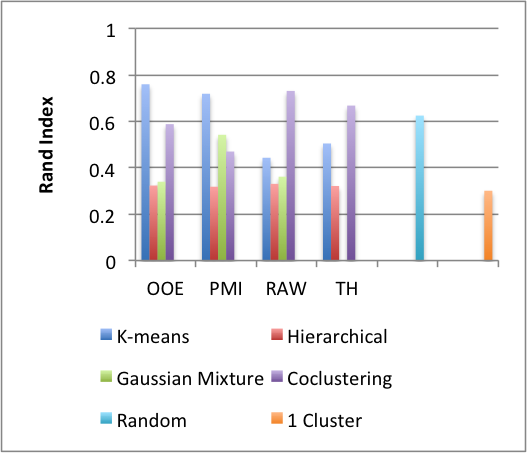
\includegraphics[width=3.5in]{RI-all.png}}
	\subfloat[]{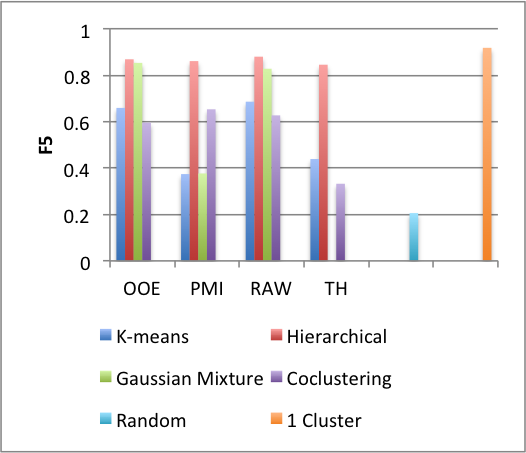
\includegraphics[width=3.5in]{F5-all.png}}	
	\caption{Clustering results for different algorithms grouped by metrics on the two measures.}
\end{figure}
		
We considered from 4 to 8 clusters, but the results were very consistent within a given metric and algorithm, so we only present results with 5 clusters. Looking closely at the results, we noticed that increasing the number of clusters didn't find substantial partitions, but simply peeled off a few elements into a very small, new cluster. Since the changes were relatively small (compared to making another large cluster), evaluation remains relatively stable.

As a baseline, I also evaluated the standard against randomly assigned clusters and everything being grouped into one large cluster. Random assignment scores fairly well on the Rand Index. Assuming that the true clusters are all of roughly even size, this shouldn't be true. However, most of the adjectives in our dataset were either relative standard or non-gradable, so there were effectively fewer clusters to predict. A single cluster scored very well on the F5 measure. Since F5 down weights false positives so much, this measure was somewhat misleading as well.

Hierarchical clustering on the whole failed. Instead of gathering large clusters together at the end, it appears to have largely been combining single elements into the mass, so the clusters ended up being single elements removed from the one large cluster. Although it appears to do well on the F5 measure, this is because of its similarity to the degenerate case of only a single cluster. This data appears to be an unfortunate case for hierarchical clustering. 

Interestingly, k-means on the OOE metric and coclustering on RAW both scored fairly well on both measures. Looking at the results by hand, we found that the clusters aligned with our expectations: they both appeared to find the gradable/non-gradable distinction and discovered other expected relationships.

We were unable to determine from an algorithmic perspective why these 2 applications worked better than any of the other approaches. With a cluster structure, we would expect that a mixture of gaussians should do at least as well as k-means, but it doesn't in our results. One hypothesis is that the space of adjectives and how they receive degree modification isn't clustered and is a more gradual transition between types. In that case, gaussians wouldn't properly capture this interaction.

The difference between coclustering on RAW and k-means on OOE may have arisen from some interaction between the metrics and dimensionality reduction. Since coclustering uses clustering for dimensionality reduction, and our application of k-means used PCA, it appears that these approaches interacted differently with OOE, which was normalized, and RAW, which was completely unnormalized. Note that k-means also performs well on PMI, another normalized measure.

One possible reason for the apparent effectiveness of coclustering on RAW is that it could've been biased significantly by the frequency of adjectives with \textit{very}. \textit{Very} is a common degree modifier, and without any normalization in RAW, the very large or very small counts for this feature may have disproportionately affected the results. The frequency of \textit{very} alone may be enough to find the gradable/non-gradable distinction.

Clustering also appears to have extracted relations other than the structure of degree modification. Since our processing didn't focus upon degree modification other than in the selection of adverbs, it is very feasible for this to have occurred.

For example, when we expanded the number of clusters to find to 20, we found clusters such as \textit{economic}, \textit{military}, \textit{physical}, and \textit{political}, which seem to be more specific to semantic relatedness or usage in newswire than degree modification. Although these are all non-gradable, it's clear that this approach has extracted more than we needed.

Another notable result is that both coclustering on RAW and k-means on OOE (our best results) put \textit{certain} and \textit{possible} in the same cluster. With degree modification, these two words are very different as they both express the same idea, except that \textit{certain} has a maximum standard and \textit{possible} has a relative standard. In this case, it's possible that it could just be semantic relatedness. Another more interesting possibility, however, is that the adverbs paired with these words are used more to assert speaker confidence than degree. For example, one can say

\begin{enumerate}
\item It's \textit{completely certain} that Stanford will win the Fiesta Bowl.
\item It's \textit{completely possible} that Stanford will win the Fiesta Bowl.
\end{enumerate}

Even though both are expressed in terms of the same dimension (possibility) and maximal degree, they don't mean the same thing. "Completely possible" refers not to maximal possibility (i.e. certainty) but instead means that the speaker is completely confident that it is possible.

Since we're interested specifically in the structure of gradable adjectives, we tried re-running the analysis over only the gradable adjectives (removing all hand-coded non-gradable adjectives from the dataset), with the results in the figure below.

\begin{figure}
	\subfloat[]{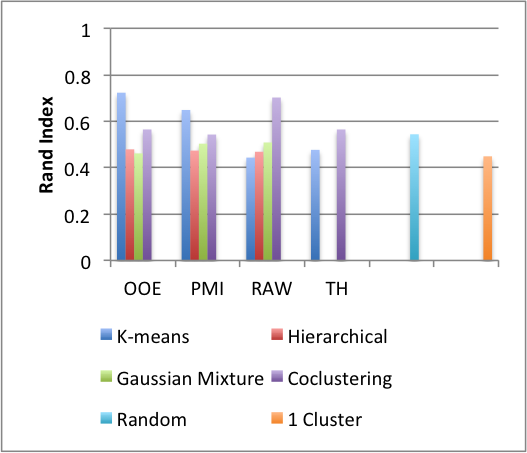
\includegraphics[width=3.5in]{RI-gradable.png}}
	\subfloat[]{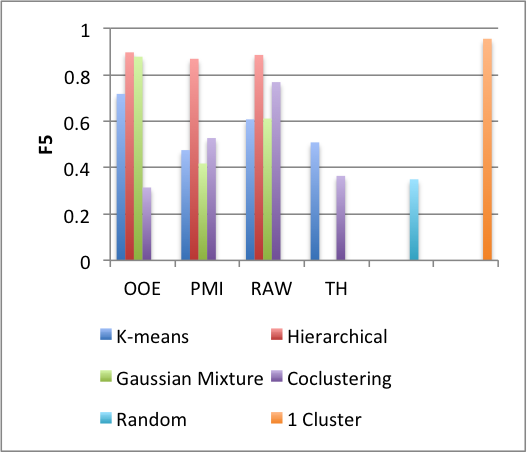
\includegraphics[width=3.5in]{F5-gradable.png}}
	\caption{Clustering results for different algorithms grouped by metric on only gradable adjectives.}
\end{figure}

Unfortunately, the results for this were less clean. The scores on both measures dropped across the board. This result wasn't unexpected as the metrics should drop after removing the easier task of clustering gradable and non-gradable adjectives. Again, k-means on OOE and coclustering on RAW scored far better than other methods.

The clusters it extracted by hand appeared less similar to the results we hoped for, though it did have some linguistic connections. For example, coclustering on RAW yielded a cluster with \textit{independent}, \textit{open}, and \textit{responsible}, which are all positive adjectives.

\section{Conclusion}
To summarize, we broke up the task of evaluating the Kennedy and McNally theory of gradable adjectives into multiple parts. First, we compared bigrams and dependencies and found them similar enough to use bigrams. Second, we considered multiple metrics to apply to the co-occurrence matrix to address different concerns we had with the data. Third, we used multiple clustering algorithms and compared the results against the predicted clusters, with varying results.

\subsection{Error Analysis}
Most of the analysis is in the sections above, but we have several broad observations to make.

First, our approach of working backwards from usage in corpus analysis to linguistic theory is somewhat tenuous. Although the data may indicate various properties, these may deal strictly with usage and have no bearing on grammaticality. There are many perfectly valid English constructions that aren't commonly used, and the normative claim that gradable adjectives should or shouldn't be able to receive particular degree modification based on frequencies is difficult.

Second and on a related note, there are quirks with the dataset. Particularly, Web 1T has been criticized for a lot of duplication of data from crawling over the same content multiple times. This may inflate the differences being observed. Also, the particular uses of the internet affect the corpus composition. One salient example is that the bigram \textit{fucking young} was very frequent in the dataset, which we infer is from questionable, adult-only content on the internet. We're uncertain about the degree to which other less provocative usage quirks might have affected our results.

Finally, the use of clustering generally can extract many different characteristics. Although we're interested in degree modification, we found examples above of other findings that can also obfuscate our intended results. Some examples include different word senses, the polarity of adjectives, and semantic relatedness.

\subsection{Future work}
Although we don't have a conclusive result on the validity of the Kennedy and McNally theory, this exploratory project allowed us to try out different approaches and explore some of the difficulties of different approaches. There are many possibilities for followup work.

First, we can complete more dependency parsing and use that as our dataset. Although we found that the data were similar, we should use the data intended for this relationship if possible. More clever schemes of combining dependency results with the size of Web 1T data may be even more helpful.

Second, we can explore different methods of establishing our standard and other properties to factor out. Currently, we only have a single coder, and given the variability in what people find acceptable, there may be some inconsistencies with general acceptability. The data could also be marked and clustered with other features, such as polarity, to understand the importance of those features as well.

Finally, we can do a better job finding only instances of degree modification by applying word sense disambiguation to the instances to discover how words are being used. One example is above with adverbs being used as either degree modifiers or expressions of speaker confidence. Another is polysemy of adjectives, where different meanings have different scale structures. Separating these cases may give cleaner data for clustering to extract patterns from.

\bibliography{ga-corpus}
\bibliographystyle{abbrv}

\end{document}  